\appendix
\section{Appendix}

\subsection{GPR-assisted basal-motion-field inversion on Argentière}\label{app:gpr}

The main analysis fixes the basal-motion parameter $\tau_{\mathrm{ref}}$ to a single
scalar, so that all three glaciers are treated identically and no thickness survey is
required. Where dense auxiliary data \emph{do} exist, however, the same differentiable
framework can exploit them to sharpen the dynamical state. Argentière is covered by
repeated ground-penetrating-radar (GPR) soundings of ice thickness
\citep{rabatel2018}; here we show that assimilating them, and relaxing
$\tau_{\mathrm{ref}}$ from a scalar into a spatial field $\tau_{\mathrm{ref}}(\mathbf{x})$
inverted jointly with the thickness, further improves the fit and surpasses the state
of the art.

The GPR soundings supply an independent thickness constraint (the second term of
Eq.~\ref{eq:da}, over the survey footprint $\Omega_{\mathrm{thk}}$) that makes the
joint inversion identifiable. The data assimilation then retrieves both the
ice-thickness field $H_{t_1}$ and the basal-motion field
$\tau_{\mathrm{ref}}(\mathbf{x})$ that together reproduce the observed surface
velocity and the GPR transects, converging within $10^2$ L-BFGS iterations
(Fig.~A1). Modelled velocities match the observations to a
root-mean-square residual of $3\,\mathrm{m\,yr^{-1}}$, and the calibrated thickness
departs from the GPR transects by RMS $=12\,\mathrm{m}$ (bias $-9\,\mathrm{m}$), of
the order of the GPR uncertainty itself. The recovered sliding field shows the
physically expected structure---enhanced along the central flowline and reduced near
the lateral margins---consistent with the finding of \citet{kneib2024} that spatial
variability in $\tau_{\mathrm{ref}}$ helps explain the observed surface velocities.

\begin{figure*}
  \centering
  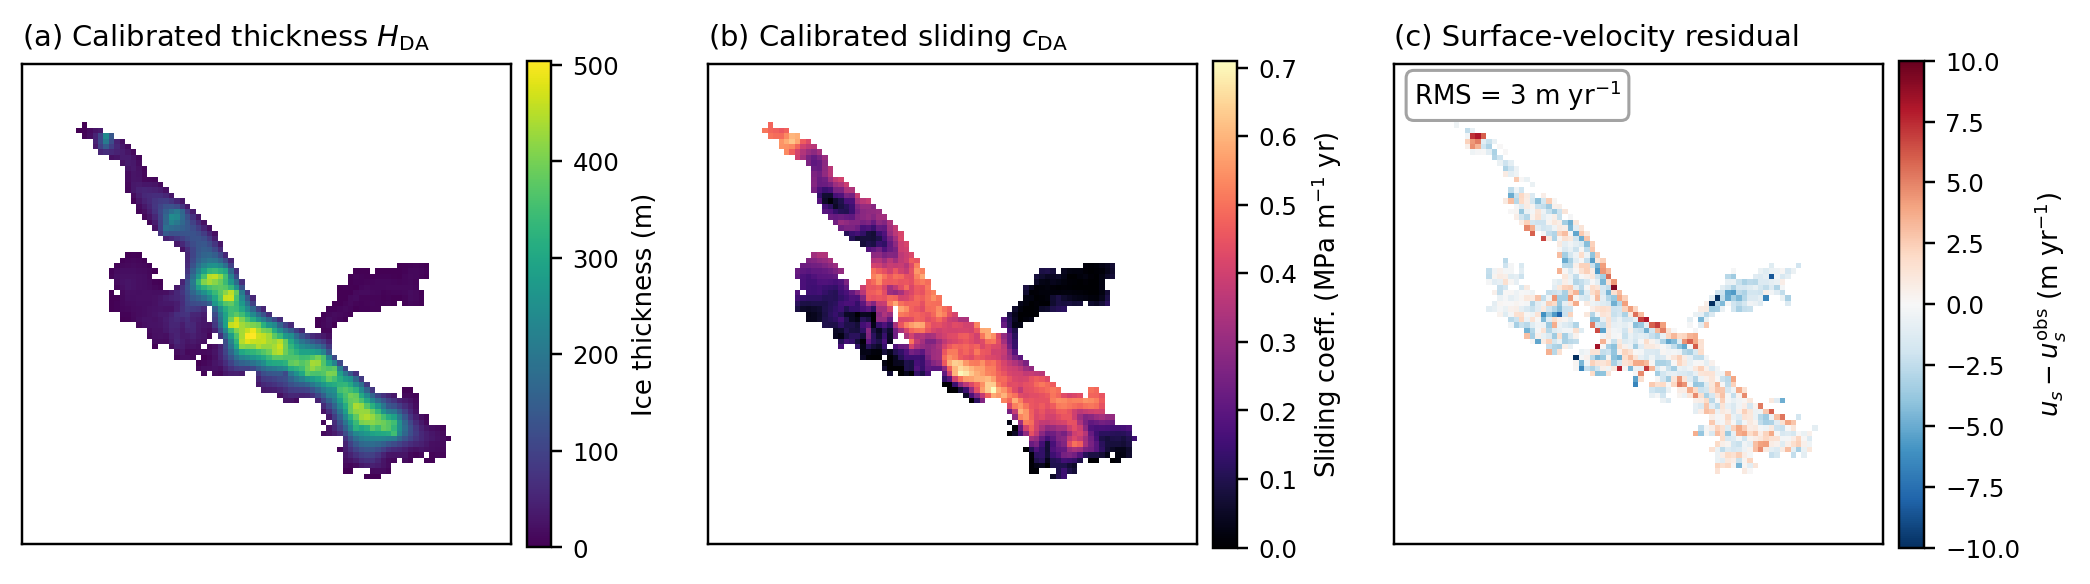
\includegraphics[width=\linewidth]{figs/argentiere_da_panel.png}
  \caption{GPR-assisted data-assimilation state on Argentière Glacier at the start
    epoch. (a)~Calibrated ice thickness $H_{t_1}$ and (b)~calibrated basal-motion
    field $\tau_{\mathrm{ref}}(\mathbf{x})$; (c)~surface-velocity residual
    $\mathbf{u}_s - \mathbf{u}_s^{\mathrm{obs}}$, near zero across the glacier
    (overall RMS $=3\,\mathrm{m\,yr^{-1}}$; white cells lack a velocity observation).}
  \label{fig:gpr-da}
\end{figure*}

Holding this calibrated state fixed, the transient inversion (2012--2021) yields the
elevation-resolved SMB profile of Fig.~A2. The simulated
end-of-window thickness matches the target across the trunk to within the
DEM-differencing uncertainty (Fig.~A3; residual RMS $=24\,\mathrm{m}$,
small and largely unbiased). Validated against the GLACIOCLIM network, the profile
reproduces the observed altitudinal pattern with a root-mean-square error of
$0.45\,\mathrm{m\,w.e.\,yr^{-1}}$---lower than the velocity-only result of the main
text ($0.65$) and below every previously published distributed reconstruction on this
site over this period, including all three baselines of \citet{kneib2024}
($0.50$--$0.85\,\mathrm{m\,w.e.\,yr^{-1}}$; Table~\ref{tab:rmse}). The residual
structured misfit in Fig.~A3(c) reflects horizontal variability within
elevation bands---notably the avalanche-fed accumulation hotspots
\citep{kneib2024}---that the one-dimensional profile does not represent.

\begin{figure}
  \centering
  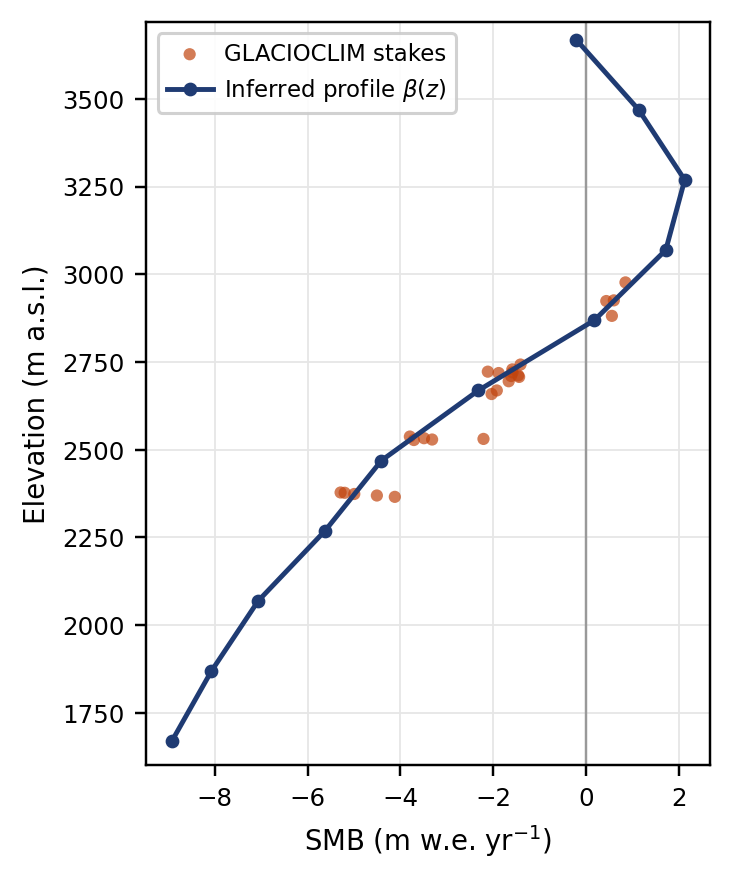
\includegraphics[width=0.7\linewidth]{figs/argentiere_smb_profile.png}
  \caption{Inferred elevation-resolved SMB profile $\beta(z)$ (blue) for Argentière
    over 2012--2021 from the GPR-assisted inversion, in water equivalent. Orange dots
    are the 2012--2021 mean GLACIOCLIM stake balances, plotted at the elevation of
    each stake. The profile spans $1670$--$3610\,\mathrm{m\,a.s.l.}$ and matches the
    stakes with $\mathrm{RMSE}=0.45\,\mathrm{m\,w.e.\,yr^{-1}}$.}
  \label{fig:gpr-smb}
\end{figure}

\begin{figure*}
  \centering
  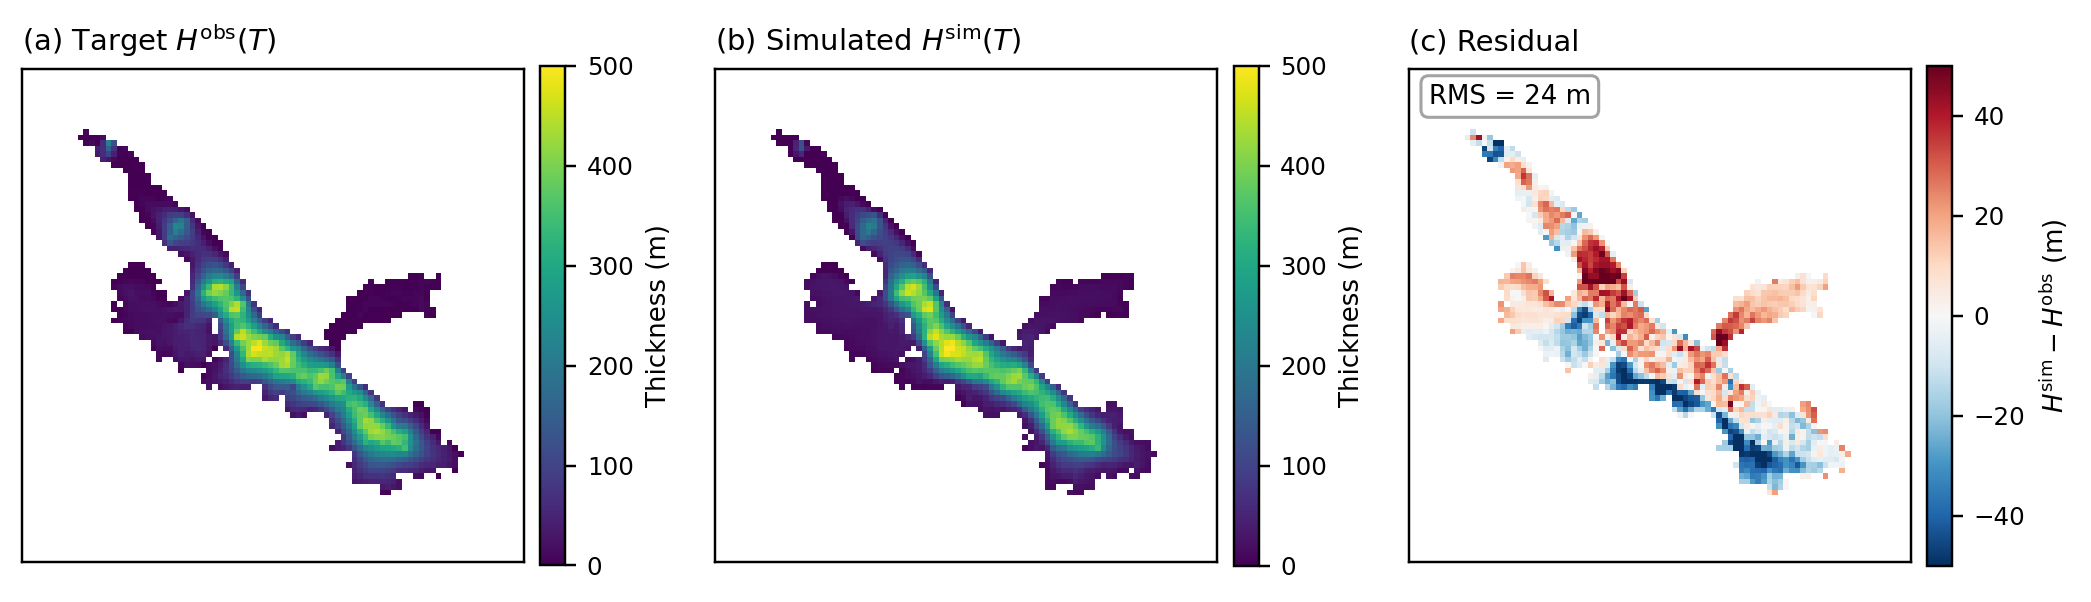
\includegraphics[width=\linewidth]{figs/argentiere_thk_comparison.png}
  \caption{End-of-window ice-thickness fit on Argentière ($t_2 = 2021$), masked to
    the glacier footprint. (a)~Target thickness $H^{\mathrm{obs}}(\cdot, t_2)$ from
    the observed surface DEM and the calibrated bedrock; (b)~simulated thickness
    $H^{\mathrm{sim}}(\cdot, t_2)$ from the forward run under the inferred SMB
    profile; (c)~their residual $H^{\mathrm{sim}} - H^{\mathrm{obs}}$
    (RMS $24\,\mathrm{m}$). The residual is small and largely unbiased; its spatially
    structured component reflects horizontal variability within elevation bands that
    the one-dimensional profile does not represent.}
  \label{fig:gpr-thk}
\end{figure*}

\subsection{Applicability to near-global elevation-change data}\label{app:hugonnet}

The fidelity of the inferred SMB is ultimately set by the quality of the input
elevation change (Sect.~\ref{sec:contribution}). The main results use dedicated
two-epoch DEMs, which deliver the highest accuracy but are not available everywhere.
Near-global elevation-change products such as that of \citet{hugonnet2021} would, by
contrast, make the method applicable to essentially any glacier. To gauge the
associated fidelity penalty, we repeat the inversion on
Rhône---chosen for its denser stake record ($n=5$ continuous-record
locations)---replacing only the geometry-change target: the observed
surface-elevation change is now the \citet{hugonnet2021} $\mathrm{d}h/\mathrm{d}t$
rate, while the velocity data assimilation and the scalar-$\tau_{\mathrm{ref}}$
ensemble search are left unchanged.

The velocity-selected coefficient ($\tau_{\mathrm{ref}}=0.12$\,MPa, again the
surface-velocity-misfit minimum) yields an inferred profile that reproduces the
stake averages with a root-mean-square error of $0.70\,\mathrm{m\,w.e.\,yr^{-1}}$
(Fig.~\ref{fig:hugonnet})---about twice the $0.32$ obtained with the
dedicated swisstopo DEMs (Sect.~\ref{sec:inferred}), yet still recovering the full
altitudinal structure and remaining well below the stationary-flux continuity
estimate ($1.79\,\mathrm{m\,w.e.\,yr^{-1}}$). The degradation is concentrated in the
upper ablation and accumulation area, and reflects the
stronger spatial smoothing and larger uncertainty of the near-global product
relative to a dedicated DEM pair. This confirms the trade-off anticipated in
Sect.~\ref{sec:contribution}: near-global elevation-change data extend the method to
almost any glacier at a fidelity cost bounded by the DEM quality, so dedicated
multi-temporal DEMs remain preferable where they exist. 

Exploring the full sliding sweep (Table~\ref{tab:hugonnet}) reinforces this: with the
Hugonnet product the surface-velocity-misfit minimum coincides with the best stake
fit, and the stake error is nearly flat across the whole low-misfit basin
($0.70$--$0.77\,\mathrm{m\,w.e.\,yr^{-1}}$), so the residual sensitivity to
$\tau_{\mathrm{ref}}$ is small next to the fidelity gap between the two
elevation-change sources.

\begin{table}
  \caption{Sensitivity of the Hugonnet-based Rhône inversion to the basal-motion
    parameter $\tau_{\mathrm{ref}}$ (at $A=78$), with the dedicated-DEM stake RMSE at
    matching $\tau_{\mathrm{ref}}$ for comparison. \emph{velsurf} is the
    surface-velocity misfit and ELA the equilibrium-line altitude; the stake RMSE is
    the validation against the $n=5$ continuous-record averages. Column minima in
    bold.}
  \label{tab:hugonnet}
  \centering
  \begin{tabular}{lcccc}
    \toprule
    $\tau_{\mathrm{ref}}$ & velsurf RMSE & ELA & \multicolumn{2}{c}{Stake RMSE (m\,w.e.\,yr$^{-1}$)} \\
    (MPa) & (m\,yr$^{-1}$) & (m\,a.s.l.) & Hugonnet & ded.\ DEMs \\
    \midrule
    0.121 & \textbf{7.56} & 3136 & \textbf{0.70} & 0.81 \\
    0.154 & 8.43          & 3096 & 0.74 & 1.25 \\
    0.199 & 9.42          & 3084 & 0.77 & \textbf{0.32} \\
    0.459 & 15.35         & 3083 & 0.73 & 0.77 \\
    0.744 & 34.77         & 3183 & 2.66 & 3.15 \\
    1.078 & 37.43         & 3422 & 2.28 & 2.06 \\
    \bottomrule
  \end{tabular}
\end{table}

\begin{figure*}
  \centering
  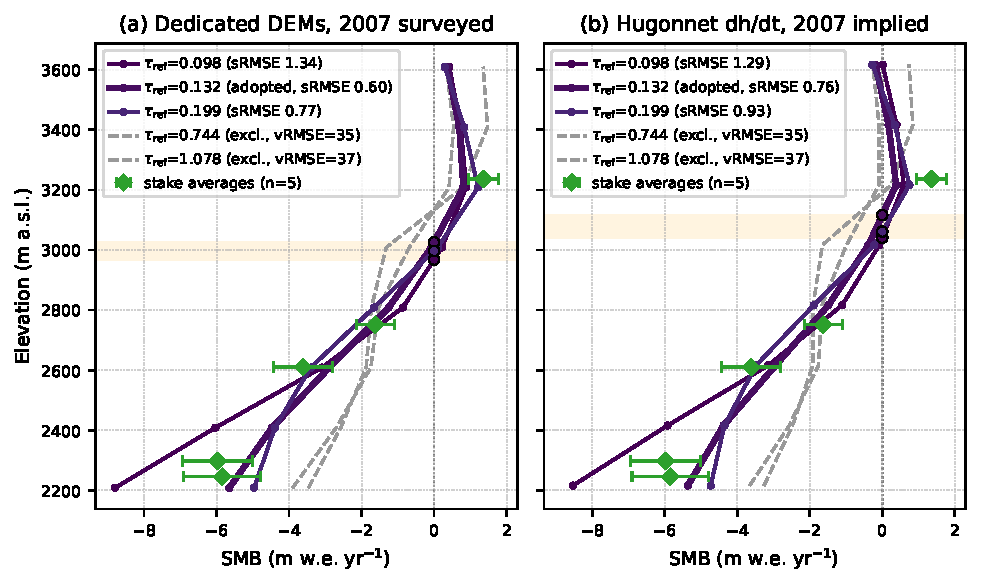
\includegraphics[width=\linewidth]{figs/fig_rhone_sens_2panel.pdf}
  \caption{Sliding-coefficient sensitivity of the Rhône inversion for the two
    elevation-change experiments: (a)~the dedicated two-epoch DEMs used in the main
    text and (b)~the \citet{hugonnet2021} $\mathrm{d}h/\mathrm{d}t$ product. Each
    panel shows the inferred SMB profile across a range of $\tau_{\mathrm{ref}}$
    (colour; the adopted profile bold with its sRMSE, and runs rejected by the
    velocity misfit dashed), the equilibrium-line-altitude band shaded, all
    validated against the same continuous-record stake averages (green diamonds).
    Both experiments recover the elevation structure, but the Hugonnet-based fan sits
    higher and is biased low in the accumulation area, giving a larger stake RMSE
    ($0.70$ vs $0.32\,\mathrm{m\,w.e.\,yr^{-1}}$).}
  \label{fig:hugonnet}
\end{figure*}
